\laborator{Моделирование процесса ректификации бинарной смеси в тарельчатой колонне}

\goal{составить математическую модель процесса ректификации бинарной смеси в тарельчатой колонне; на ее основе разработать алгоритм численного решения и, используя язык программирования Mathcad, провести моделирование колонны.}

\subsubsection{Теория}
Разделение жидких смесей ректификацией на практически чистые компоненты или на фракции различного состава является широко распространенным процессом химической технологии. Разделению подвергаются смеси, состоящие из компонентов с неограниченной и ограниченной взаимной растворимостью. Каждому классу этих смесей соответствуют характерные условия равновесия кипящей жидкой фазы и образующихся из нее паров, отображаемые диаграммами фазового равновесия жидкость~-- пар.

При кипении жидкой смеси концентрация низкокипящего компонента в образующихся парах больше, чем в жидкой фазе. При частичной конденсации образовавшейся паровой фазы, конденсироваться в большей степени будут высококипящие компоненты, а остаток пара будет обогащен низкокипящими компонентами. Это позволяет разделить исходную жидкую смесь с любым числом компонентов на любое число фракций различных составов путем частичного испарения этой смеси и конденсации образующихся паров. Такой процесс называется дистилляцией, получаемые конденсаты – дистиллятами, а неиспарившаяся часть жидкой смеси – кубовым остатком. 

Для более четкого разделения исходной жидкой смеси на узкие фракции или чистые компоненты прибегают к многократному чередованию процессов испарения и конденсации. Этот сложный процесс, называемый ректификацией, осуществляется в колонных аппаратах при противотоке жидкости и пара. Восходящий поток пара при каждом контакте со стекающей жидкой смесью обогащается низкокипящими компонентами за счет частичной конденсации высококипящих и частичного испарения низкокипящих. При достаточном числе таких контактов пар будет уходить из верхнего сечения колонны с преимущественным содержанием низкокипящих, а жидкость уйдет из нижнего сечения колонны с преимущественным содержанием высококипящих компонентов.

Процесс ректификации осуществляется в большинстве случаев в противоточных колонных аппаратах с контактными элементами (насадки, тарелки). Схема типовой ректификационной установки непрерывного действия представлена на рисунке \ref{fig:rect.scheme}.

\begin{figure}[h]
	\begin{center}
		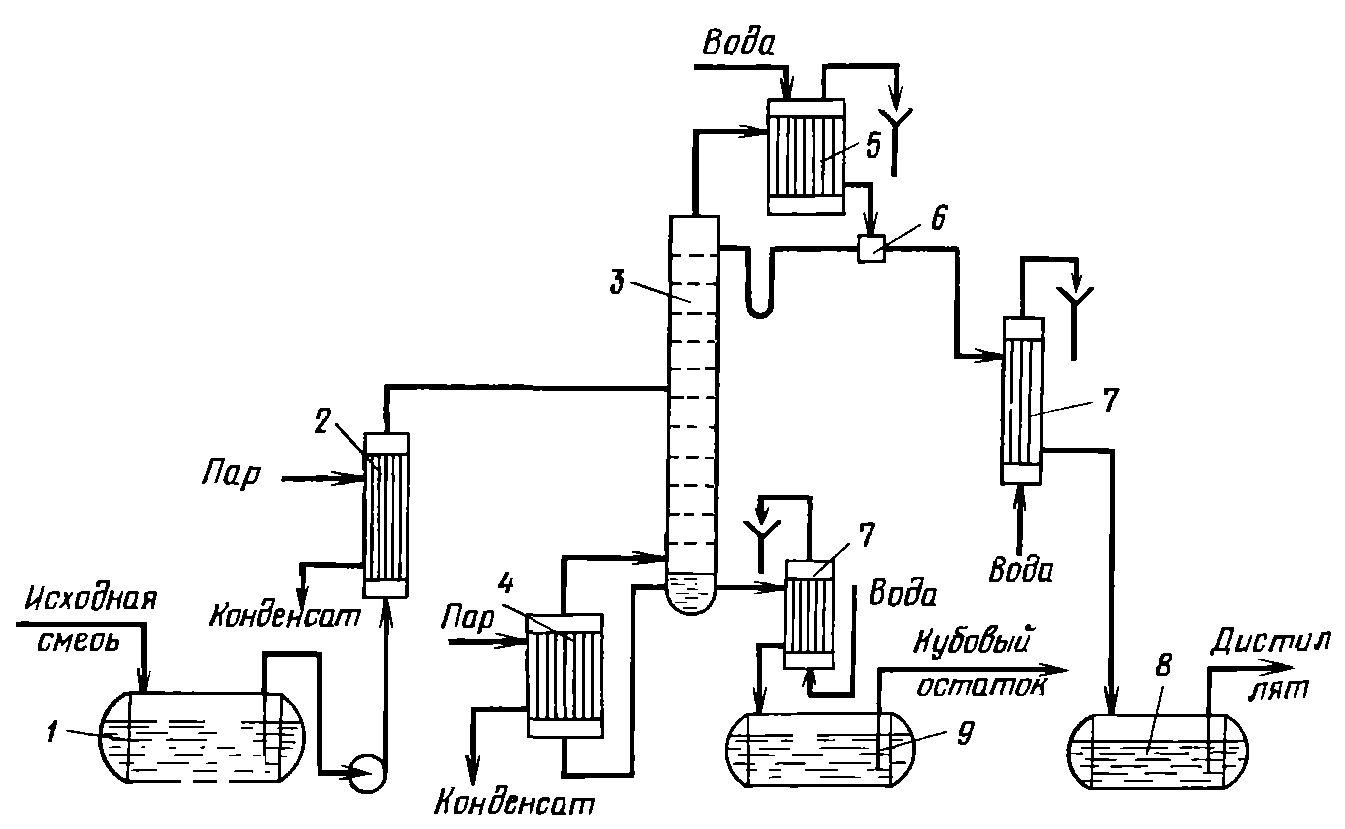
\includegraphics[width=\textwidth]{scheme.png}
	\end{center}
	\caption{Схема ректификационной установки непрерывного действия:1 --- емкость для исходной смеси; 2 --- подогреватель; 3 --- колонна; 4 --- кипятильник; 5 --- дефлегматор; 6 --- делитель флегмы; 7 --- холодильник; 8 --- сборник дистиллята; 9 --- сборник кубового остатка} \label{fig:rect.scheme}
\end{figure}


Исходную смесь подают в то место ректификационной колонны 3, в котором состав жидкой фазы наиболее близок по составу к смеси, поступающей в колонну на разделение. Подача питания обеспечивает непрерывность проведения процесса ректификации. Место ввода исходной смеси, нагретой до температуры кипения в подогревателе 2, называют тарелкой питания, или питательной тарелкой. Положение тарелки питания для ввода исходной смеси специально рассчитывается. Поток пара, поднимающегося по ректификационной колонне, поддерживается испарением кубовой жидкости в кипятильнике 4, а поток жидкости, текущей по колонне сверху вниз, флегмой, образующейся при конденсации выходящих из колонны паров в дефлегматоре 5. Отношение расхода флегмы $Ф$ к расходу отбираемого дистиллята $Р$ называют флегмовым числом $R$ (т. е. $R = Ф/Р$).

Из всей схемы ректификационной установки (рис. \ref{fig:rect.scheme}) при моделировании процесса ректификации рассматриваются только сама ректификационная колонна 3, кипятильник 4 и дефлегматор 5. Данные аппараты оказывают влияние на ход процесса разделения \cite{klinov-mm2009}. Остальное оборудование (в основном это теплообменники) определяется в последующем, исходя из результатов расчета колонны. При технологическом расчете массообменных аппаратов должны быть определены их основные размеры: диаметр, характеризующий производительность аппарата, и рабочая высота, отражающая интенсивность протекающего в нем процесса.

Расчет диаметра аппарата производится по уравнению расхода:
\begin{equation}
	Q=S w_0
\end{equation}
где $Q$ --- объемный расход пара, скорость которого определяет площадь поперечного сечения колонны; $w_0$ --- фиктивная скорость пара; $S$ --- площадь поперечного сечения аппарата. Обычно нижняя часть ректификационной колонны работает при большем орошении по сравнению с верхней, поэтому иногда (для повышения эффективности работы верхней части) необходимо рассчитывать верхнюю и нижнюю части колонны отдельно.

Высота массообменного аппарата определяется в зависимости от того, является контакт фаз в нем непрерывным или ступенчатым. При непрерывном контакте фаз высоту аппарата можно найти на основе уравнения массопередачи или его модификации, выразив высоту аппарата с помощью единиц переноса.

Для расчета высоты аппарата через число ступеней в аппаратах со ступенчатым контактом фаз необходимое число ступеней определяется графическими или аналитическими методами. Графические методы имеют ограничения, так как они применимы только при расчете бинарной ректификации. Аналитические методы применимы как в случае бинарной, так и многокомпонентной ректификации.

Одним из аналитических методов расчета ректификационной колоны является метод расчета от тарелки к тарелке, в котором последовательно определяются расходы материальных потоков и их составы на каждой ступени разделения. В самом простом виде данный метод имеет следующие допущения:
\begin{itemize}
	\item жидкость на тарелке полностью перемешана;
	\item молярные расходы пара и жидкости по колонне не изменяются;
	\item в дефлегматоре и кипятильнике не происходит изменения соответственно состава пара и жидкости.
\end{itemize}

В результате сделанных допущений из уравнения материального баланса и массопереноса для каждого компонента на тарелке получают уравнения, устанавливающие зависимость между составами пара и жидкости покидающими тарелку. 
Спецификой процесса ректификации является сопряженность процессов массо- и теплопереноса, что приводит к некоторым последствиям, усложняющим анализ и расчет данного процесса. Некоторые из них кратко рассмотрены ниже:
\begin{itemize}
	\item иногда возможно существенное изменение физических свойств сред по высоте колонны, что может повлиять не только на скорость массопереноса, но даже и на величину поверхности контакта фаз (ухудшение или улучшение смачиваемости насадки, изменение размеров пузырьков и т.д.). Последнее обстоятельство связано в основном с изменением поверхностного натяжения жидкости как следствие изменения ее состава и температуры;
	\item допущение при анализе и расчете ректификационных колонн равенства молярных теплот испарения компонентов иногда может дать достаточно большие отклонения. Анализ этих возможных эффектов следует проводить в каждом конкретном случае.
\end{itemize}

\begin{wrapfigure}{R}{0.4\textwidth}
	\begin{center}
 		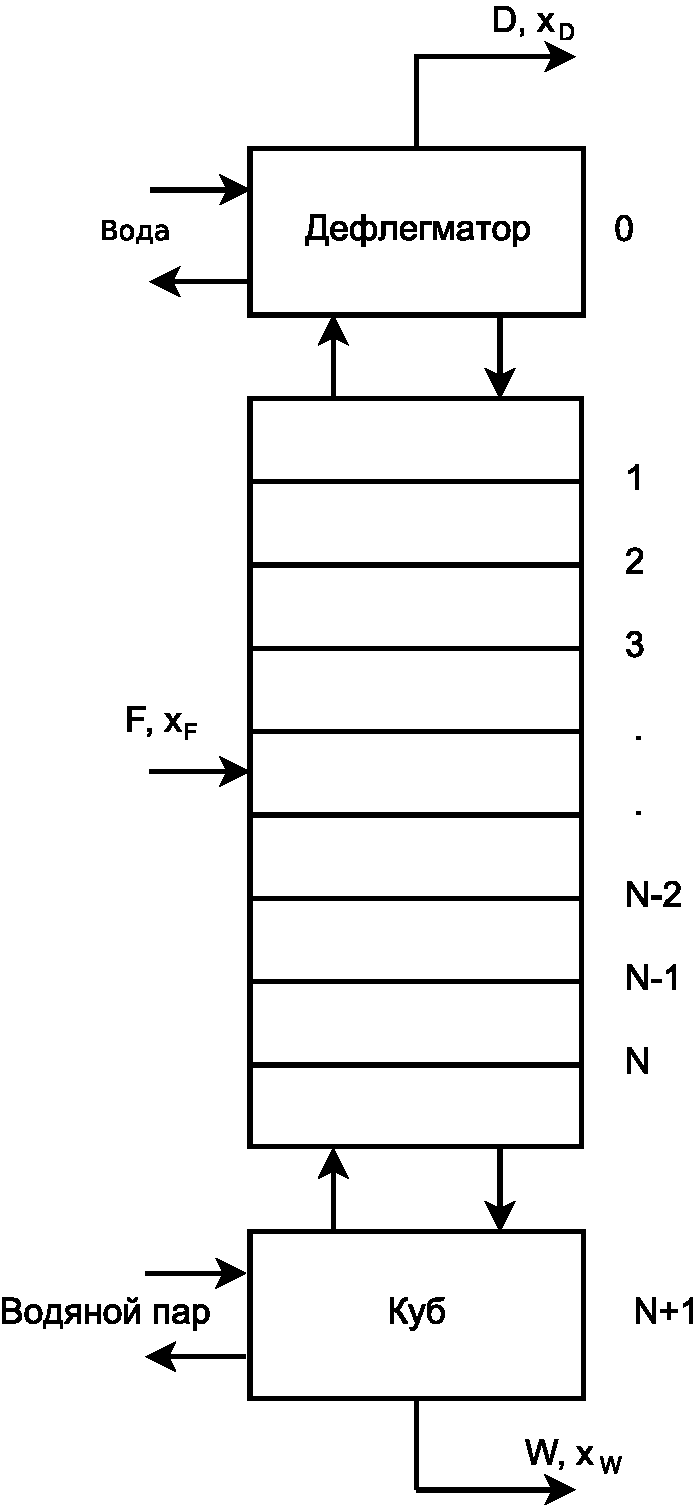
\includegraphics[width=0.48\textwidth]{colomn.pdf}
	\end{center}
	\caption{Схема ректификационной колонны} \label{fig:rect.col}
\end{wrapfigure}
 
Вместе с тем следует отметить, что все названные выше эффекты обычно ускоряют процесс массопереноса. Поэтому при расчете процесса ректификации это, как правило, дает запас производительности и эффективности колонны.

Тарельчатые колонны относятся к аппаратам со ступенчатым контактом фаз и для их расчета используют метод расчета «от тарелки к тарелке». Каждой тарелке присваивают порядковый номер, нумерацию ведут сверху вниз (рисунок \ref{fig:rect.col}). При расчете ректификационной колонны необходимо учитывать дефлегматор и кипятильник, которым также присваивают номера: дефлегматору --- нулевой; кипятильнику --- $N + 1$. При рассмотрении ректификационных колонн для разделения бинарной смеси применим однонаправленный расчет (снизу вверх или сверху вниз) колонны.


На первом этапе оценки возможности проведения процесса разделения смеси используется метод теоретической тарелки. Полученные при этом результаты позволяют дать предварительную оценку необходимого количества ступеней разделения и определить основные режимные параметры процесса давление, флегмовое число и т.д., в последующем эти результаты уточняются. 

При рассмотрении ректификационной колонны в рамках метода теоретической тарелки, основное влияние на точность расчета оказывает правильность определения условий фазового равновесия пар – жидкость. 

Условия равновесия двух фаз $n$~-- компонентной системы, когда температура в каждой фазе одинаковы, определяются следующей системой уравнений:
\begin{equation}
	\left\lbrace 
	\begin{gathered} 
	p^{ж}(T, x_1, x_2, \ldots, x_n-1)=\\=p^{п}(T, y_1, y_2, \ldots, y_n-1)\\
	\mu_k^{ж}(T, x_1, x_2, \ldots, x_n-1)=\\=\mu^{п}_k(T, y_1, y_2, \ldots, y_n-1) 
	\end{gathered} 
	\right.
\end{equation}
где $\mu$ --- химический потенциал, $п$ и $ж$ --- паровая и жидкая фазы, соответственно. Химический потенциал и давление системы определяются следующим образом:
\begin{equation}
	\mu_i(T,x)=\mu_i^0 (T) +RT \ln(\gamma_i x_i)
\end{equation}
\begin{equation}
	p=\sum\limits_{i=1}^{n} p_i= \sum\limits_{i=1}^{n} \gamma_i p_i^0 x_i
\end{equation}

В этом случае для расчета условий фазового равновесия кроме давления паров чистого компонента при заданной температуре $p_i^0(T)$ и идеальногазовой составляющей химического потенциала $\mu_i^0(T)$, необходимо определять коэффициенты активности $\gamma_i$ в зависимости от температуры, давления и состава.

При расчете процессов разделения для упрощения задачи перепад давления (гидравлическое сопротивление) по высоте ректификационной колонны принимают равным нулю. Таким образом, процесс разделения обычно моделируется при фиксированном давлении, а профиль температур по колонне определяется в ходе расчета исходя из состава смеси в колонне. В действительности же, давление в кубе колонне всегда больше чем вверху колонны на величину ее гидравлического сопротивления. 

При расчете условий фазовых равновесий используется концепция избыточной энергии Гиббса, которая заключается в том, что уровень энергии Гиббса для смеси превышает величину характерную для идеального раствора при тех же значениях температуры, давления и состава. Выражения для определения избыточной мольной энергии Гиббса:
\begin{equation}
	G^E=RT(x_1\ln (\gamma_1) +x_2 \ln(\gamma_2))
\end{equation}

Некоторые уравнения для избыточной мольной энергии Гиббса $G^E$ в отличие от уравнения Маргулеса содержат температуру в явном виде (NRTL и др.) \cite{rid1982,yelles1989}. Однако из этого вовсе не следует, что константы таких уравнений не зависят от температуры. Приводимая явная температурная зависимость --- всего лишь приближение и ни в коем случае такие уравнения для $G^E$ не являются точными.

Кроме того, основное влияние температуры на равновесие пар~-- жидкость оказывается через давление паров чистых компонентов $p^0(T)$. Коэффициенты активности зависят как от температуры, так и от состава, и температурную зависимость коэффициентов активности можно считать слабо выраженной по сравнению с зависимостью давлений паров чистых жидкостей от температуры. Для типовой смеси подъем температуры на 10$\mathrm{^\circ}C$ приводит к возрастанию давлений паров чистых жидкостей в $1.5 - 2$ раза, а изменение коэффициентов активности составит скорей несколько процентов, т.е., величину, которая часто меньше погрешности эксперимента. Таким образом, если не происходит сильного изменения температуры, часто при расчетах равновесия пар~-- жидкость можно пренебречь влиянием температуры на $G^E$.
 
Таким образом, на достоверность моделирования процесса разделения значительное влияние оказывает правильность определения температуры на каждой ступени контакта фаз.

В общем виде математическая модель процесса разделения, протекающая на N--ой ступени (рисунок \ref{fig:rect.col}), запишется в виде:
\begin{equation} \label{eq:rect.equation}
\left\lbrace 
\begin{gathered} 
E=\dfrac{y_{N+1}-y_{N}}{y_{N+1}-y^*}\\
L(x_{N-1}-x_N)=G(y_N-y_{N+1})
\end{gathered} 
\right.
\end{equation}
где $Е$ --- коэффициент полезного действия (или эффективности) по Мэрфи; $L$, $G$ --- мольные расходы жидкой и паровой фаз по высоте колонны, соответственно; $y^*$ – равновесная концентрация в паровой фазе. Данную модель необходимо дополнить уравнением, определяющим равновесные концентрации компонентов в паре:
\begin{equation}
	y_i^*=\dfrac{p_i^0 \gamma_i x_i}{p}
\end{equation}
и выражением для определения давления паров чистых компонентов $p^0(Т)$ и коэффициентов активности $\gamma(x,T)$.

Для решения системы уравнений \eqref{eq:rect.equation} необходимо определить мольные расходы паровой и жидкой фаз по высоте колонны. Для этого первоначально необходимо из материального баланса определить расходы дистиллята $D$ и кубового остатка $W$:
\begin{equation}
	W = \dfrac{F (x_D - x_F)}{x_D - x_W},
\end{equation}
\begin{equation}
	D = F - W,
\end{equation}
индексами $D$, $W$, $F$ обозначены составы дистиллята, кубового остатка и исходной смеси соответственно. 

Рабочее флегмовое число определяется исходя из минимального флегмового числа:
\begin{equation}
	R_{min}  = \dfrac{x_D - y^*_F}{y^*_F - x_F}.
\end{equation}
Предложено несколько вариантов определения флегмового числа, исходя из минимизации затрат на проведение процесса. В данной лабораторной работе предлагается пользоваться заданным значением коэффициента избытка флегмы $\beta$:
\begin{equation} 
	R = R_{min} \beta
\end{equation}
Всю колонну можно разбить на 2 части, разделяемые тарелкой питания. В верхней части поток жидкой фазы будет равен:
\begin{equation}
	L_{u} = D R \dfrac{M^x_u}{M_D},
\end{equation}
в нижней:
\begin{equation}
	L_{d} = DR \dfrac{M^x_d}{M_D} + F \dfrac{M^x_d}{M_F}
\end{equation}
В верхней части поток газовой фазы равен:
\begin{equation}
G_u = D(R+1)\dfrac{M^y_u}{M_D},
\end{equation}
в нижней:
\begin{equation}
G_d = D(R+1)\dfrac{M^y_d}{M_D},
\end{equation}
где $M$ --- молярные массы смеси, нижние индексы $u$ и $d$ обозначают средние значения в врхней и нижней части соответственно, верхние индексы $x$ и $y$ обозначают фазу.



\subsubsection*{Вопросы для самоконтроля}
\begin{enumerate}
\item Что понимается под процессом ректификации, в чем его отличие от дистилляции? 
\item Что такое флегмовое число и каково его влияние на процесс разделения?
\item Что называется теоретической тарелкой?
\item Что такое эффективность по Мэрфри и как она влияет на высоту ректификационной колонны?
\item Какие допущения используются при расчете процесса ректификации?
\end{enumerate}


\subsubsection{Пример задания}
Используя язык программирования MathCad провести расчеты простой тарельчатой ректификационной колонны непрерывного действия, предназначенной для разделения $F = 5$ т/ч исходной бинарной смеси, содержащей  $x_F = 34$~\% масс. низкокипящего компонента. Разделение проводится при атмосферном давлении. Исходная смесь поступает в аппарат при температуре кипения. Требуемый состав дистиллята $x_D = 91$~\% масс, куба --- $x_W = 0.5$~\%. Коэффициент избытка флегмы $\beta = 1.25$. КПД тарелок $E = 0.7$.
Для расчета использовать метод расчета от тарелки к тарелке. Допущения при расчете:
\begin{enumerate}
	\item куб колонны --- полный испаритель;
	\item дефлегматор --- полный конденсатор.
\end{enumerate}

В качестве исходной смеси принять смесь согласно своему варианту из лабораторной работы 5, и использовать полученные там функции для составов паровой и жидкой фаз.


